\documentclass{llncs}
\usepackage[english]{babel}
\usepackage[T1]{fontenc}
\usepackage[utf8]{inputenc}
\usepackage{graphicx}
\usepackage{epstopdf}
\usepackage{color}
\usepackage{comment}
\usepackage{amsmath}
\usepackage{subcaption}
\usepackage{float}
\usepackage{xspace}
\captionsetup{compatibility=false}
\captionsetup{singlelinecheck=off}
\captionsetup{justification=centering}

\newfloat{post}{th}{qt}
\floatname{post}{Post}

\newfloat{equationBlock}{th}{qt}
\floatname{equationBlock}{Equation}


\pagestyle{plain}
\newcommand{\todo}[1]{{\color{red}TODO:~#1}}
\newcommand{\nr}{~\todo{Reference}~}
\newcommand{\nto}{\emph{NTO}\xspace}
\newcommand{\acme}{\emph{ACME}\xspace}
\newcommand{\boxedTex}[1]{{\fbox{\begin{minipage}{10 cm}~#1\end{minipage}}}}
\newcommand{\textoverline}[1]{$\overline{\mbox{#1}}$}

\title{Noise-To-Opportunity Conversion for Social Media Posts}
\author{Stefan Bunk, Dimitri Korsch, Daniel Kurzynski}

\institute{Hasso Plattner Institute, Potsdam, Germany\\
  \email{\{firstname.lastname\}@student.hpi.uni-potsdam.de}
}
\begin{document}

\maketitle

\begin{abstract}
%!TEX root = ../paper.tex

This paper introduces a new approach for companies to find potential customers in social networks.
By listening to noise from social network posts, we identify users, which express a demand for a certain product.
We achieve this identification with a two-stage text categorization classifier:
First, we detect whether the post  expresses a demand for some product in general.
Second, we detect, which product the post is about.
By using the company's brochures, we minimize the integration effort of our system.
However, this approach is difficult, because brochures differ from social network posts in style and length and only a few brochures exist for each product.
By employing feature selection and document sampling we are able to cope with these issues.
Our evaluation has shown the practicability of this approach and supports our decisions for a two-stage classifier, document sampling, and strict feature selection.

\end{abstract}

%!TEX root = ../paper.tex

\todo{
	\\
	\textbf{Questions} \\
	\begin{itemize}
		\item Base paper on algorithm or dataset?
		\item Tagging app?
	\end{itemize}
	\textbf{Final checks} \\
	\begin{itemize}
		\item "data set" vs "dataset"
		\item Check headline capitalization
		\item Check capitalization after hyphen
	\end{itemize}
}

\todo{Talk about 2-step classifier and show figure one on first page}

\section{Introduction}
\label{sec:introduction}

Recent years have shown a trend for companies from buying standalone software with big service contracts to buying small cloud products, also known as software as a service (SaaS).
Software is licensed on a subscription and per-use basis and is hosted on the vendors's servers.
Vendors of such software are now able to set the subscription fees dynamically according to usage time, company size, or revenue.
For the customer companies, this allows to scale easily when the company grows or declines or does not need the services for a certain time span.

These new possibilities increased the set of potential customers for software vendors.
As Dubey and Wagle~\cite{dubey2007delivering} said, ``buyers have more flexibility to switch vendors and perhaps fewer headaches in maintaining the software".
Especially young companies are more likely to buy SaaS, as it gives them the flexibility to adapt to the growth of the company in the future.
So, rather than being restricted to a small range of companies, for example only big enterprise companies or only young startups, vendors can sell their products to all kinds of companies.
However, this introduces a new problem for the salesmen: due to the sheer amount of possible customers, it is harder to find those, who are likely to buy the product.
When only a few companies are available, salesmen can just inquire personally and try to sell their products.
In the new setting, it becomes harder and more time-consuming to find potential customers.
% New startups do not need to make a decision about whether to buy a big, standalone software straightahead, or first buying a smaller system and only later upgrade to a bigger system.

We propose a new approach to find potential customers by automatically recommending users, who ask for product recommendations in social networks.
Social networks are platforms, where users can post status updates, ask questions, start discussions, or get recommendations.
A special type of social network, so called business-oriented social networking services like LinkedIn\footnote{http://www.linkedin.com/} or Xing\footnote{http://www.xing.com}, especially lend themselves to building business relations and asking for professional advice.
There, users ask for opinions and recommendations on products.

This offers a huge possibility for companies to identify potential buyers.
Rather than booking advertising time in television or advertising banners on news websites, they can target their salesman on persons, who are more likely to buy a product.
It is a basic truism from marketing, that it is best to target those potential customers, who are already predisposed towards the product. \nr

Thus, it makes sense for companies to find these people looking for advice.
However, the large amount of daily status updates every day makes it infeasible to identify this posts manually.
According to LinkedIn, there were 350 users in 2014, each of them posting three posts each week \todo{Random numbers: Check actual values}.
The sheer amount of this shows, that technical assistance is needed.

At the moment, this mostly happens by providing a search engine on the posts.
Salesmen need to manually find good search terms, enter them in the network's search field and then scan the results for potential buyers.
This requires expertise on the hand of the salesman to find good search terms and tweak them accordingly.
Furthermore, scanning through the result lists is cumbersome and tedious.
Also, it is simply impossible to search through a large set of posts, say over a million, and find the best possible customers, where best means that there is a high probability of a deal.

We propose an approach, which is based on automatic text classification to identify relevant posts for a salesman.
Therefore, we employ techniques of supervised machine learning to categorize posts.
We call our approach \emph{Noise to Opportunity}, as we automatically filter the best selling opportunities from the large and diverse set of potential social network posts.

To classify posts, the machine learning requires to have labeled posts to use as training data for the learning algorithm.
As this training data does not exist, it would need to be created manually by the salesmen.
However, this is not feasible for a company, as it takes precious time for tagging post from the salesmen, in which they could actually sell products.
Therefore, we propose an approach, which automatically uses the company's brochures and advertising texts for learning.
A company usually has some set of advertising material, flyers, or presentation slides, where they promote their own products.
Based on this material, we automatically learn to distinguish between products, and then propose posts with selling opportunities to the salesman.
The architecture of our system is illustrated in Figure~\ref{fig:figureone}.

\begin{figure}
	\label{fig:figureone}
	\begin{center}
		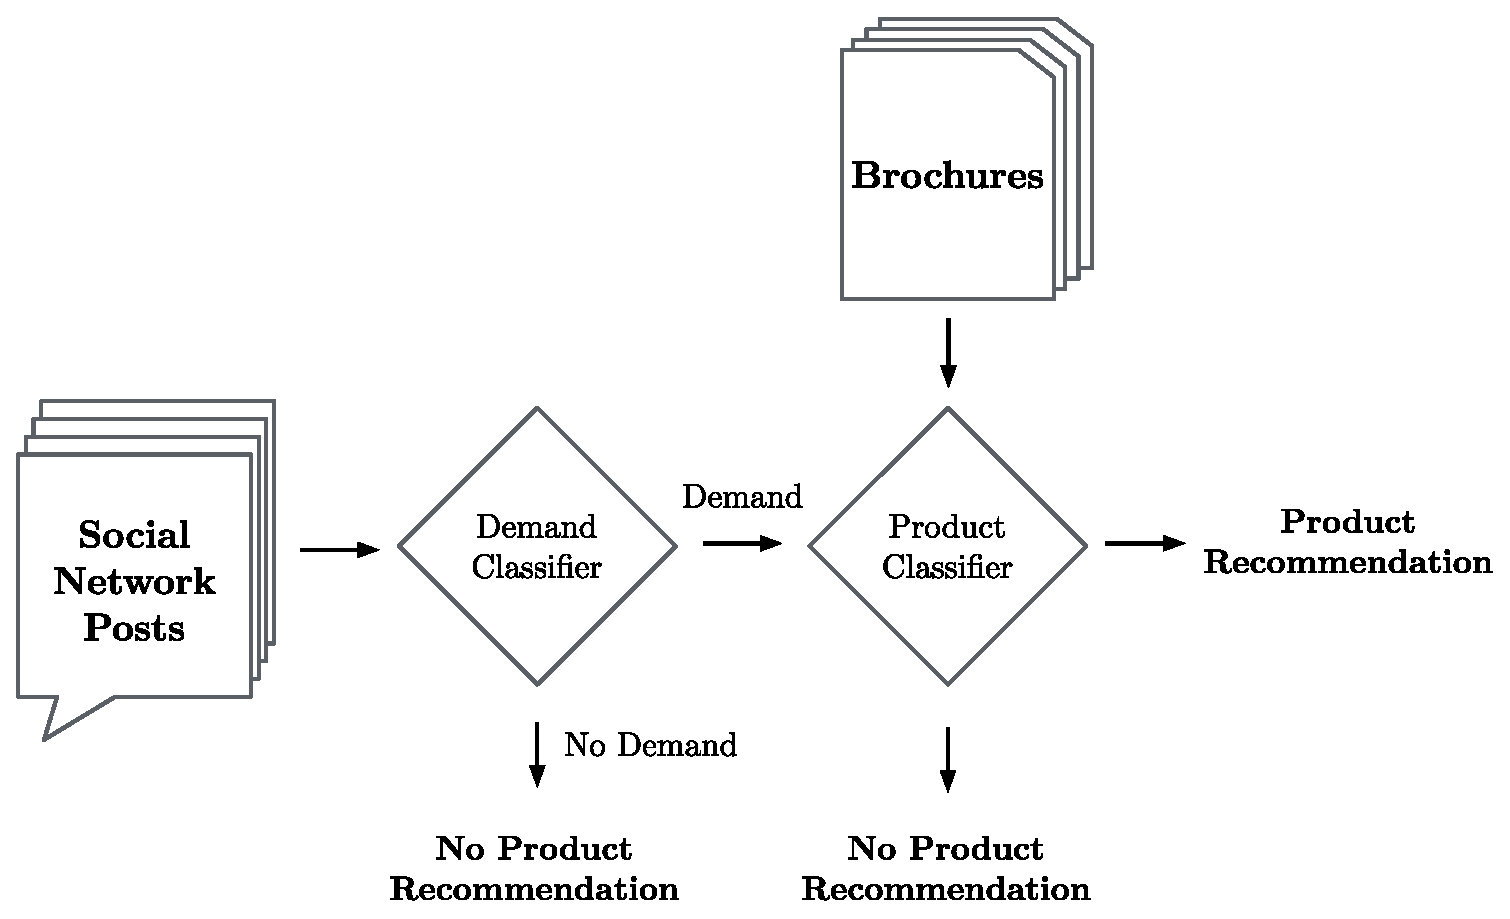
\includegraphics[width=0.7\textwidth]{figures/nto_workflow.eps}
	\end{center}
	\caption{Together, a demand classifier training from social network posts and a product classifier trained from marketing material form a classification-model for unseen posts.}
\end{figure}

Yet, this approach introduces new problems.
Firstly, there are not many documents to learn from.
The number of brochures per product is usually far below one hundred.
To overcome this small corpus problem \todo{correct name?}, we employ feature selection to only select the most relevant words and ignore the noise.
Secondly, if a user posts something about a certain product, this does not automatically allow the conclusion, that the user is actually interested in buying the product.
Therefore, we introduce a two-staged classifier, which first determines the demand of a user, and then determines, whether the user posts about a product.
This approach allows to capture, whether the user actually needs the product.

Section~\ref{sec:background} gives a formal problem definition and shows related work.
Section~\ref{sec:concept} shows our two-staged classification and how we use feature selection to overcome the small corpus problem.
Section~\ref{sec:implementation} shows the implementation of both the demand and the product classifier.
It also presents the best configuration for the algorithm.
In Section~\ref{sec:evaluation}, we evaluate our approach.
Section~\ref{sec:conclusion} summarizes and shows our planned future work. \todo{I don't think it is planed!}

\begin{itemize}
	\item outline your contributions (not your paper$\ddot\smile$)
\end{itemize}


%!TEX root = ../paper.tex

\section{Text Classification in Marketing}
\label{sec:background}

This section shows related work from text classification and recommender systems.
Then we give a formal problem definition and show challenges, that have to be solved.

\subsection{Related Work}
The text classification task has been researched already in many other works.
Yang et al.\cite{yang1999re} have compared the performance of different text classifiers in their paper.
They tested linear classifiers, rule-based classifiers, k-nearest-neighbours and na\"ive bayes classifiers.
In their evaluation, the different classifiers did not differ by more than five percent.
McCallum et al. \cite{mccallum1998comparison} specifically focus on na\"ive bayes classifiers.
They found out, that na\"ive bayes classifiers perform good on small corpus and vocabulary sizes.

In the area of automatic product recommendations, research has focused on displaying ads in search engines.
Mehta et al.\cite{mehta2007adwords} present an algorithm to find ads to display given a user's search terms.
However, for search engines the input mostly is only a few words, while we use entire posts.
The concept is also different, because companies directly place bids on certain keywords.
This leads to a large preselection already.

There is also a wide research on recommender systems. 
Especially the content-based recommender systems~\cite{lops2011content} are similar to our problem.
Content-based recommender systems use the content to identify items ''similar to those a given user has liked in the past''~\cite{lops2011content}.
We also recommend posts to salesmen.
However, we do not have a history of posts.
We use marketing materials as similarity measure.

Furthermore, we focus not on recommending products to users automatically but on identifying posts for salesmen.
This is why we need to be sure that a recommended post expresses a need for a specific product.
Therefore, we think, that this paper represents a good beginning for the research in this field of text classification.


\subsection{Problem Definition}
\label{sec:background-problem}

In this section we formally define the \emph{noise to opportunity problem}.
We also talk about problems that occur while solving the task.

Let \acme be an example company that offers a wide range of different products.
As in every company, there are salesmen who want to get in contact with potential buyers of these products.
For different products, there are different salesman responsible and different potential buyers.
To find these buyers we help \acme to identify people on business networks, who seem to have a need for products offered by \acme.

We call our approach noise to opportunity conversion or the \nto problem.
We choose the word noise because of the amount of daily status updates in business networks, which makes it infeasible to listen to all of them.
Also, status updates are usually quite diverse: people write posts, which differ in length, use different words for the same thing, use  different abbreviations or even invent new words.
Nevertheless, there are many posts which are a good opportunity to get in contact with people who want to buy products a salesman's company offers.

Posts~\ref{post:demand-and-product}, ~\ref{post:demand-only}, and~\ref{post:product-only} show how posts in such business-oriented social networks look like.
We have to decide which of these posts are written by potential customers of \acme.

\begin{post}
	\centering
	\boxedTex{
		Hi, I'm looking for CRM advice.
		We're a gaming company, currently focused on a Slot Machine game on iOS and Android.
		We're in the process of finding a CRM platform to help us manage our player base.
		Do you have any recommendations?
	}
	\caption{The user wants to buy a new product, here a software for customer relationship management (CRM). Assuming that \acme sells this type of product, the system should make a recommendation.}
	\label{post:demand-and-product}
\end{post}

\begin{post}
	\centering
	\boxedTex{
		Hi, I am looking for your advice.
		Which car should I buy next?
		Do you have any recommendations
	}
	\caption{The user wants to buy something, but assuming that \acme does not sell cars, the system should not make a recommendation.}
	\label{post:demand-only}
\end{post}

\begin{post}
	\centering
	\boxedTex{
		Please, join our demo tomorrow. We give you an overview of different CRM systems.
		We also show how you can improve your customer relations to increase your sales.
	}
	\caption{The post is about a product offered by the company, but the user does not want to buy the product. The system should not make a recommendation.}
	\label{post:product-only}
\end{post}

We would only recommend Post~\ref{post:demand-and-product} to \acme.
Post~\ref{post:demand-and-product} expresses that the user is searching for a new customer relationship managment (CRM) system.
This product is offered by \acme.
In Post~\ref{post:demand-only}, the user is searching for a product.
However, this post is uninteresting for \acme because cars are not in \acme's product portfolio.
In contrast, Post~\ref{post:product-only} is about CRM systems, but the user is not interested in a new CRM system.
Therefore the post should not be shown to a salesman.

The decision, whether to recommend a post, depends on two characteristics:
First, the post should express that users needs something, e.g. a certain product.
Second, the product needed by the user should be offered by \acme.

Formally, the problem can be defined as:
Let $p \in POSTS$ be a post from a business-oriented social networking service.
Let $PRODUCTS$ denote the set of a company's products.
Then, the problem can be modelled as a function $\nto$, such that:
\begin{displaymath}
	\nto: POSTS \to PRODUCTS \cup \{NONE\}
\end{displaymath}
This function can also be seen as an assignment of a post to a salesman.
Usually, one salesman is not responsible for all products of \acme, but rather specializes in a few.
If the \nto function outputs $CRM$, then the post is shown to one of the CRM salesmen for review.

A classification of a post $p \in POSTS$ is $correct$, if $\nto(p)$ is indeed the product that seems to be needed by the user who posted $p$ or $NONE$ if the user does not need a product offered by the company \acme.
If $p$ is a post, then we propose $p$ to a salesman if $\nto(p) \neq NONE$.

We can optimize our algorithm for two use cases: helping salesmen find relevant posts or displaying advertisement automatically.
For helping salesmen it is important to have a high precision.
If we recommend a post to salesmen we want to be confident, that our recommendation is correct.
A high precision reduces the amount of unnecessary work.
For displaying advertisements automatically the recall should be high.
It is important to recommend products to as many users as possible.
It is acceptable if some of the recommendations are not correct.

In the following sections we explain how we approached the problem of approximating the~\nto function.
We achieve this by learning a classifier from a sample data set.
The classifier needs a data set with some classified documents.
Classified means, that they are already tagged with respect to whether our \nto function should recommend a product or not.
This is called a gold standard.
However, salesmen do not want to read through hundreds of posts to tag them manually.
Therefore, we need a different data source.
We decide to use advertisement brochures describing \acme's products.
As a consequence of using brochures a problem arises from the theoretical learning perspective.

From a probabilistic point of view the instances are drawn from an unknown distribution.
Learning means to find a function, which minimizes the expected loss with respect to this distribution~\cite{trafalis2000support}.
In our approach, training works on brochures, while later we want to classify social network posts.
They are not drawn from the same population which means that the distributions are different.
Therefore, the resulting function might not be the optimal with respect to classifying posts.
To overcome this, we take a closer look on the differences between brochures and posts:

 \begin{itemize}
 	\item
		\emph{Non-user perspective}:
		Brochures are written from the perspective of salesmen.
		However, we want to classify on user-written social network posts.
		As Post~\ref{post:product-only} illustrates, simply finding posts similar to the brochures is not sufficient, as we also need to consider whether the user actually wants feedback and recommendations.
	\item
		\emph{Document mismatch}:
		Brochures are written with a different intent as posts.
		There is a crucial difference in writing style and word choice between posts.
		In brochures there are words from the marketing domain.
		Also, brochures are much longer.
		Usually, they are at least one page long while social network posts consist only of a few sentences.
	\item
		\emph{Small corpus}:
		Using brochures in the learning phase is a problem, because there are only a few brochures for each product.
 \end{itemize}


%!TEX root = ../paper.tex
%Concept is more general where as implementation is solving problems with the specific domain/data
\section{Concept}
\label{sec:concept}
We now present our approach to the \nto problem.
The next section details our two-staged classification approach.
We then talk about what features we select and how we approach the three problems outlined above.

\subsection{Two-staged classification}
As presented in Section~\ref{sec:background-problem} there exist the problem, that brochures are not written from the user perspective.
We called this the \emph{non-user perspective problem}.
In fact, there also exist two concepts in the posts.
These concepts are orthogonal to each other and are shown below.

First, users might express a need, demand, or interest for some product or not.
This might be a product of our company or not.
Typical phrases, taken from an experiment on our example data set (see Section~\ref{sec:evaluation}), for this concept are:
\begin{center}
	\textit{need, hi, looking for, recommend, please, anyone, appreciate, thank you}
\end{center}
We call this the \emph{demand classification}:
\begin{align*}
	\mathbf{demand}&: POSTS \longrightarrow \big\{ \operatorname{``demand''}, \operatorname{``no-demand''} \big\}
\end{align*}

The second concept is about which product the user is talking about in the post.
Here, the decision needs to be made whether this is a product of the company or not.
In the latter case, we are not interested in the post anymore.
Depending on the actual product, the relevant words vary greatly.
The following words are relevant words for a customer relationship managment software, also taken from our example data:
\begin{center}
	\textit{customer, sales, crm, b2b, consumer, salesforce, organization, account}
\end{center}

We call this the \emph{product classification}:
\begin{align*}
	\mathbf{product}&: POST \longrightarrow  PRODUCT \cup \big\{ NONE \big\}
\end{align*}

The intersection of the most relevant words for demand and product classification is the empty set.
This observation shows, that these concepts are independent of each other and should be treated separately.
If a post is about a product of the company, that does not necessarily mean, that the system should make a recommendation and vice versa.
Demand posts and posts about one of ACME's product have different characteristica, which should be represented in the system's architecture.

Therefore, we split the \nto problem in two subproblems: given a post $p \in POSTS$ we first identify, whether the posts expresses a demand for any product in general.
If this is true, we then check whether we can actually categorize the post into one of ACME's products.
All together, given $demand$ and $product$, we can define \nto:

\todo{Reference it!}
\begin{equationBlock}
	\label{equation:two-stages}
	\begin{alignat*}{3}
	  &\mathbf{NTO}: && ~POSTS && \longrightarrow PRODUCT \cup \big\{ NONE \big\} \\
	  &\mathbf{NTO}: && ~~p   && \longmapsto \begin{cases}
		    product(post)~~~~~~~\text{if }~demand(post) = \operatorname{``demand''} \\
		    NONE~~~~~~~~~~~~~~~\text{otherwise}
	   \end{cases}
	\end{alignat*}
	\caption{Defining \nto via two-staged classification.}
\end{equationBlock}

In our system, both $demand$ and $product$ are implemented by two independent text classification algorithms.
We are using supervised machine learning for this.
Supervised learning requires tagged training samples to draw conclusions on unseen test samples.

The training data for the $demand$ classifier comes from posts from social media networks.
This requires manually classifying posts into ``demand'' and ``no-demand''.
We did this manually for a sample of social network posts.
However, the demand classification does not change for different companies or products.
It is independent from the product classification, which is why companies do not need to supply training data for the demand classification.
Rather, they can use a prebuilt demand classifier.

The training data for the $product$ classifier needs to be supplied in form of brochures and/or marketing material for the different products.
Each brochure must be assigned to one product.
There can be more than one product.
The system then automatically learns from the brochures.
Figure~\ref{fig:figureone} illustrates the architecture of the system.

Learning demand and product categorization as two concepts with different classifiers also helps overcome data sparsity issues.
The number of posts that actually are asking for a product of the company is usually very low.
In our example data set, these posts only cover less than 1~\% of the posts, whereas demand posts alone occur with 8.35~\% probability and product documents alone with 25.48~\%.
If the machine learning would work directly on the positive examples, this would introduce a high data skew.
The number of positive training samples would be at least a magnitude lower than the number of negative samples.
This skew has been shown to harm the performance of machine learning systems significantly \cite{monard2002learning,guo2008class}.

However, even with two classifiers, the number of positive samples is much lower than the number of negative examples.
Therefore, we employ techniques of feature selection and training data sampling, which are shown in the next two sections.

\subsection{Feature Selection}
\label{sec:feature-selection}
As we use supervised machine-learning for the text categorization, we need to define features, which are good for predicting a demand and a certain product.
The general approach to features in text classification is the bag-of-words model \cite{yang1997comparative,zhang2010understanding}.
This model treats each text as a multiset of words in the text.
This approach loses the text order, but keeps the information about the frequency of words.
Our classifiers are based on a bag-of-word approach.

Because we have both the \emph{problem of document mismatch} and the \emph{problem of a small corpus}, we use a strict feature selection to avoid any overfitting to the training data and selecting the wrong words.

For the demand classifier, the first observation is, that there no specific words for no-demand posts.
Almost every randomly selected post does not express a demand, and it could be about any topic.
Therefore, we choose to select only words, which express a demand (e.g. ``recommend'', ``help'', ``looking'', ``need'').
The intuition is, that if enough of demand words occur, we classify a demand, otherwise a no-demand.
To identify these words we run two statistics on the data:
which words are more likely to occur in demand-posts, and which words are more likely to not occur in no-demand posts.
\begin{figure}
	\label{eq:demand_feature_selection}
	\begin{alignat*}{3}
		&demand\_prob\_with(w) &&= \dfrac{
		 		\#~\operatorname{demand}~posts~\mathbf{with}~w
			}{
				 \#~\operatorname{demand}~posts
			}
			\\
		&no\_demand\_prob\_with(w) &&= \dfrac{
		 		\#~\operatorname{no-demand}~posts~\mathbf{with}~w
			}{
				 \#~\operatorname{no-demand}~posts
			}
			\\
		&demand\_fraction\_with(w) &&= \frac{
				demand\_prob\_with(w)
			}{
				no\_demand\_prob\_with(w)
			}
			\\[2mm]
			\hline
			\\[0.1mm]
		&demand\_prob\_without(w) &&= \dfrac{
		 		\#~\operatorname{demand}~posts~\mathbf{without}~w
			}{
				 \#~\operatorname{demand}~posts
			}
			\\
		&no\_demand\_prob\_without(w) &&= \dfrac{
		 		\#~\operatorname{no-demand}~posts~\mathbf{without}~w
			}{
				 \#~\operatorname{no-demand}~posts
			}
			\\
		&demand\_fraction\_without(w) &&= \frac{
				no\_demand\_prob\_without(w)
			}{
				demand\_prob\_without(w)
			}
	\end{alignat*}
	\caption{The demand feature selection is based on the two functions $demand\_fraction\_with$ and $demand\_fraction\_without$, which select words, that are an indication for a demand post.}
\end{figure}
We select those words with the highest $demand\_fraction\_with$ and the highest $demand\_fraction\_without$.
The final demand words is the set union of these two sets.
These words indicate a demand: if they do occur, then that is a sign for a demand post, if they do not occur, then that is a sign for a no-demand post.
Using this approach we can overcome the \emph{small corpus problem} for the demand posts.

For the product classifier we use a classical tf-idf\cite{sparck1972statistical} feature selection.
Often, only a few keywords indicate membership to a product class.
Tf-idf helps to find these words, while ignoring words that may occur in every brochure, like the company name, stop words or generic words.
% The demand classifier is trained on social network posts and also predicts on social network posts.

% document mismatch --> strict feature selection
% small corpus --> training data generation

\subsection{Training data generation}

As said before, the number of brochures is usually quite low, hence there is not much training data.
Also, there exists a mismatch between the posts and the brochures.
One part of this document mismatch is, that brochures are usually much longer than social network posts, which often only contain two or three sentences, while brochures span over pages.
Hence, a natural approach is to split one long brochure into several smaller brochures, which both creates more training data and adapts the document length closer to the post's document length.


%!TEX root = ../paper.tex

\section{Implementation}
\label{sec:implementation}

\begin{itemize}
	\item Present data set?
	\item Do classifier optimization
	\item For the concrete data set, how do we split concretely.
\end{itemize}

\subsection{Evaluation data set}
\label{sub:initial_data_set}
We built a prototype of an \nto system.
This prototype is build for the products of a German software company called SAP.
SAP is the biggest software vendor in Europe and builds software for both small and large enterprises.
SAP provided us with nearly 100 brochures about four SAP software products, which are explained in Table~\ref{table:products}.
We chose LinkedIn as the business-oriented social network, as it is the biggest and most popular platform.
We crawled approximately 19,000 LinkedIn posts.
Unfortunately three forth of the brochures are in German language and the LinkedIn posts are written in English.
To solve the language mismatch, we have translated the documents with an automated translator and replaced the German brochures with its translations.
Additionally we have added some book descriptions from Amazon about these products to enlarge the training set.
As already mentioned in the previous sections to extend our training set further, we split the brochures and the Amazon descriptions.
With the help of the splitting the training set grows to 994 document, which we use for the training of the product classifier.

\subsection{Manual annotation of the LinkedIn posts}
\label{sub:manual_annotation_of_the_linkedin_posts}

At the moment, there exists no data set for a demand classification, which can be used for learning and evaluation purposes: we tagged some post manually.
We used an active learning \nr approach to create the gold standard for both training and evaluation:
first, we randomly tagged some posts, then we build a basic classifier, which repeatedly asked for those instances, where it was most unsure about.
Then it reran the classification and asked again.
We have implemented a tagging web app which implements the active learning.
All together, we tagged about 350 LinkedIn posts, both for demand and product.
In an initial step, each post was tagged at least twice to avoid misclassifications because of the opinion of one tagger.
If there were conflicts between the tagging decisions, a third person was tagging again to solve the conflict.
To evaluate the demand classifier, we use a ten-fold cross validation.
Since we have brochures for the products, on which we can learn, we used all annotated posts exclusively for the evaluation in the case of the product classifier.


\subsection{Demand Classifier}

Furthermore, we added the following handcrafted \todo{Better word} features, which have been show to increase the overall performance:
\begin{itemize}
	\item Number of questions in the post. Demand posts usually have more questions.
	\item Number of imperatives in the post. Demand posts usually have more imperatives like ``Please help me out" or ``Give me advice".
	\item Whether an e-mail address was given in the post. Demand posts often give an e-mail address to send answers to.
\end{itemize}

\subsection{Product Classifier}
To be done.

\subsection{Choosing splitting algorithm}
How we split.


%!TEX root = ../paper.tex

\section{Evaluation}
\label{sec:evaluation}

The following sections show the evaluation of our approach.
We start with defining relevant evaluation measures and then evaluate our two classifiers and relevant design decisions.

\subsection{Evaluation measures}
\label{sub:evaluation_measures}
We will use the following measures to evaluate our approach:
As already mentioned in a previous section, the demand classifier can be optimized for either precision or recall, depending on the use case.
Additionally, we look at the overall precision of both, the demand and product classifiers.
Therefore, we consider three values:

\begin{align*}
	\emph{Precision of the demand classifier}: P_{demand} 			&= \frac{correct~predicted~demands}{predicted~demands} \\
	\emph{Recall of the demand classifier}: R_{demand} 				&= \frac{correct~predicted~demands}{all~demand~posts} \\
	\emph{Overall precision of the demand and product classifier}: P_{all} &= \frac{correct~predictions}{all~predictions} \\
\end{align*}

This measures capture the most important aspects of our system: If we predict a demand, how likely is it really a demand post ($P_{demand}$), and how many of all demand posts can we actually find ($R_{demand}$).
Finally, the overall precision ($P_{all}$) of the demand classifier is usually quite high because of the data skew in the demand tagging.
A tagger, which always returns ``no-demand'' will have an overall precision of \todo{percent}, as seen in Table~\todo{NUMBER}.
However, we left this in for the sake of completeness and take all three measure in count to evaluate demand classifier performance.
Since there is no such data skew in the product classifier, the overall precision is sufficient to describe the product classifier performance.


\begin{figure}
	\begin{center}
		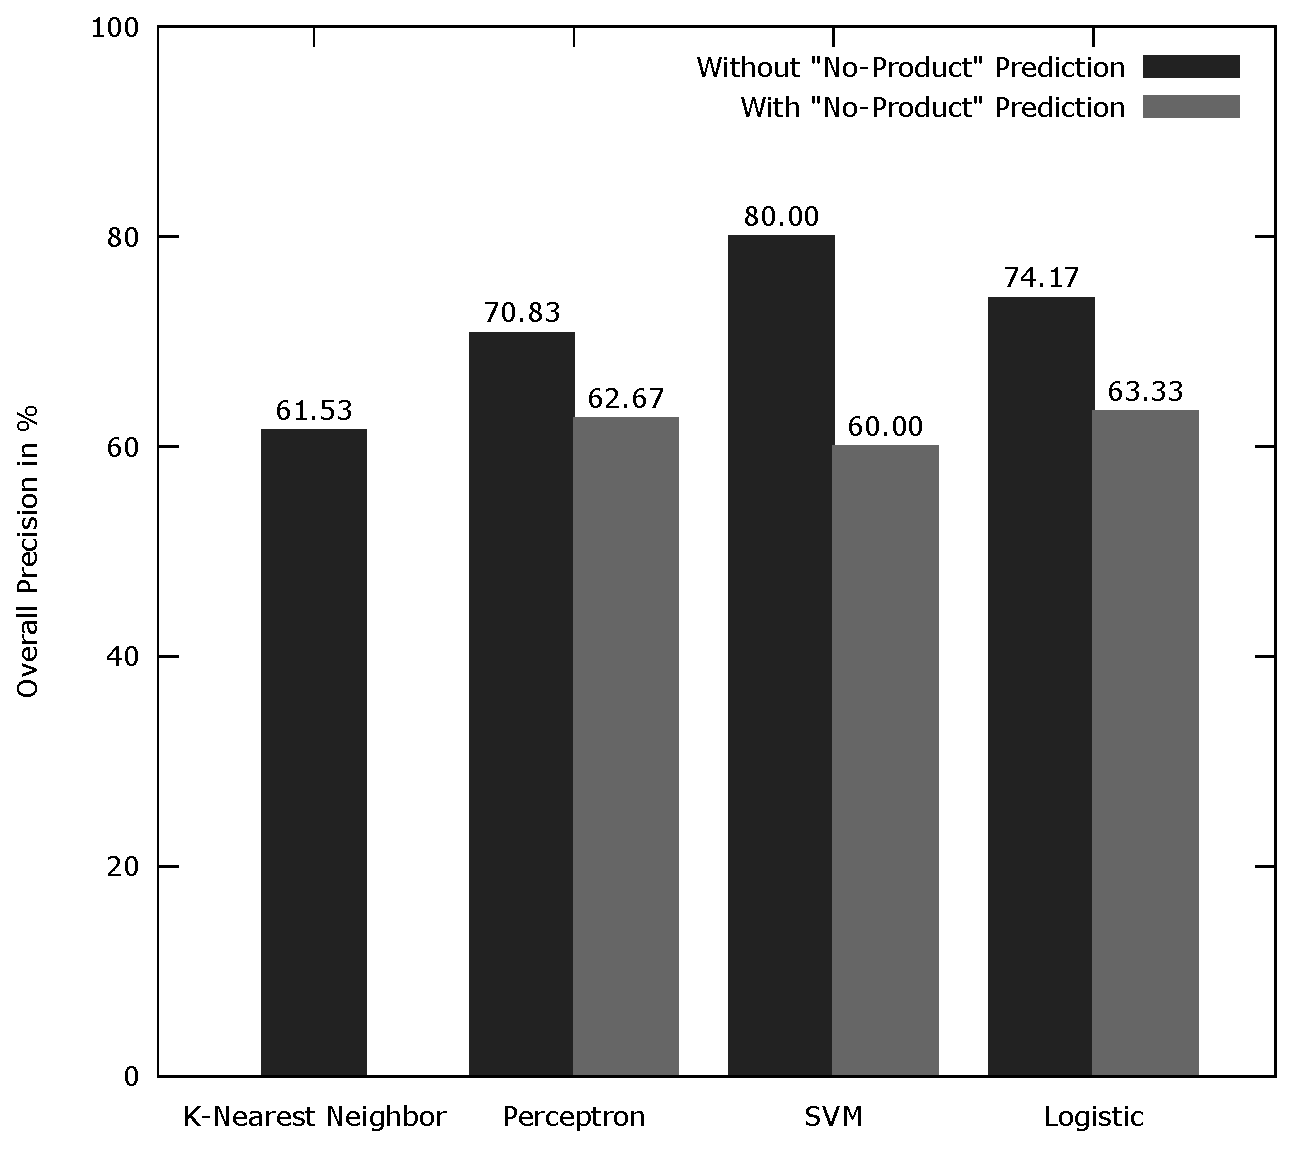
\includegraphics[width=0.7\textwidth]{figures/product_eval.eps}
	\end{center}
	\caption{Comparison of different classifiers and different classification modes}
	\label{fig:product_eval}
\end{figure}

\begin{figure}
	\centering
	\begin{subfigure}[t]{0.5\textwidth}
		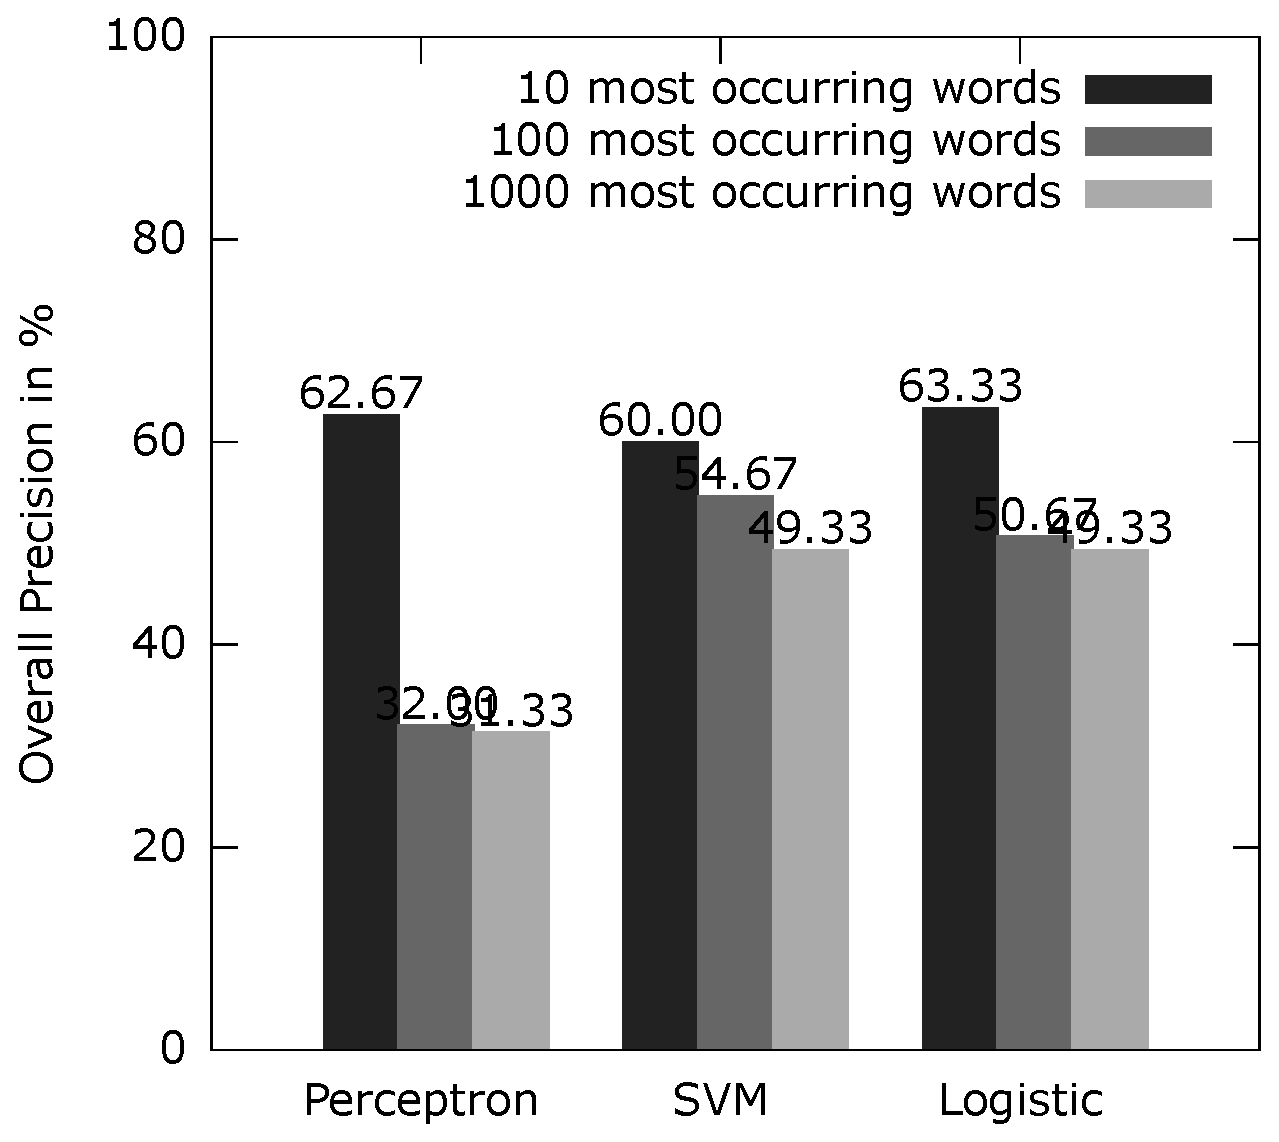
\includegraphics[width=\textwidth]{figures/product_feature_selection_with_none.eps}
		\caption{with ``no-product'' prediction}
	\end{subfigure}~
	\begin{subfigure}[t]{0.5\textwidth}
		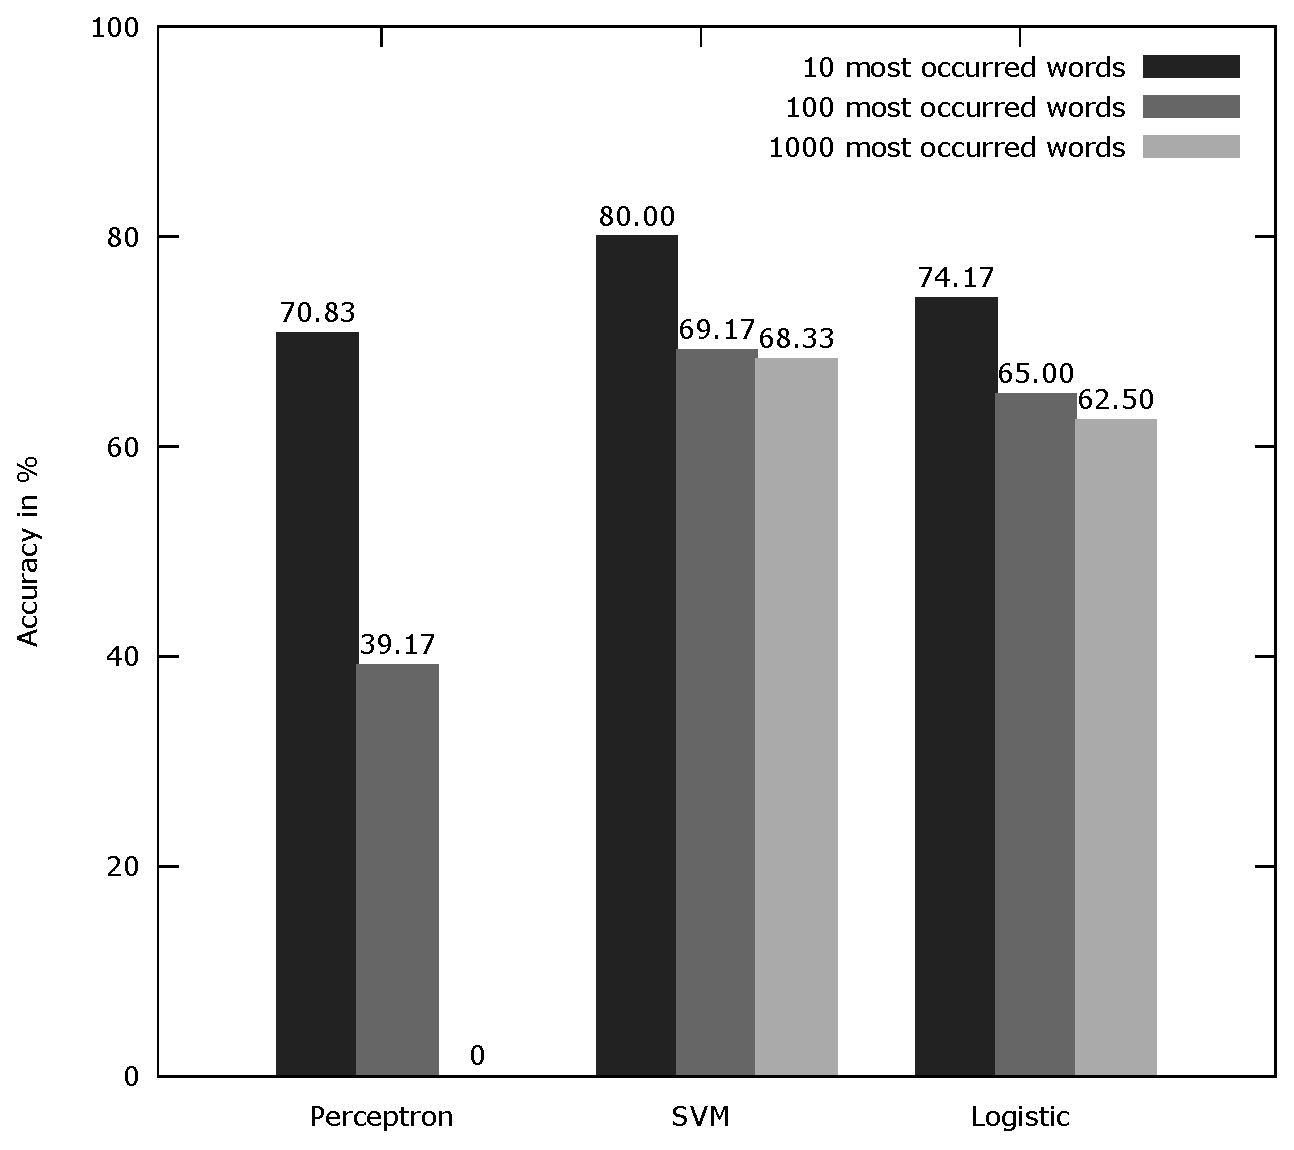
\includegraphics[width=\textwidth]{figures/product_feature_selection_without_none.eps}
		\caption{without ``no-product'' prediction}
	\end{subfigure}
	\caption{Feature Selection: comparison of ten-, 100- and 1000-most occurred words selected as tf-idf features}
	\label{fig:product_feature_selection}
\end{figure}

\todo{Find better descriptions for data}
\todo{Avoid glich of values in bars}

\begin{figure}
	\centering
	\begin{subfigure}[t]{0.5\textwidth}
		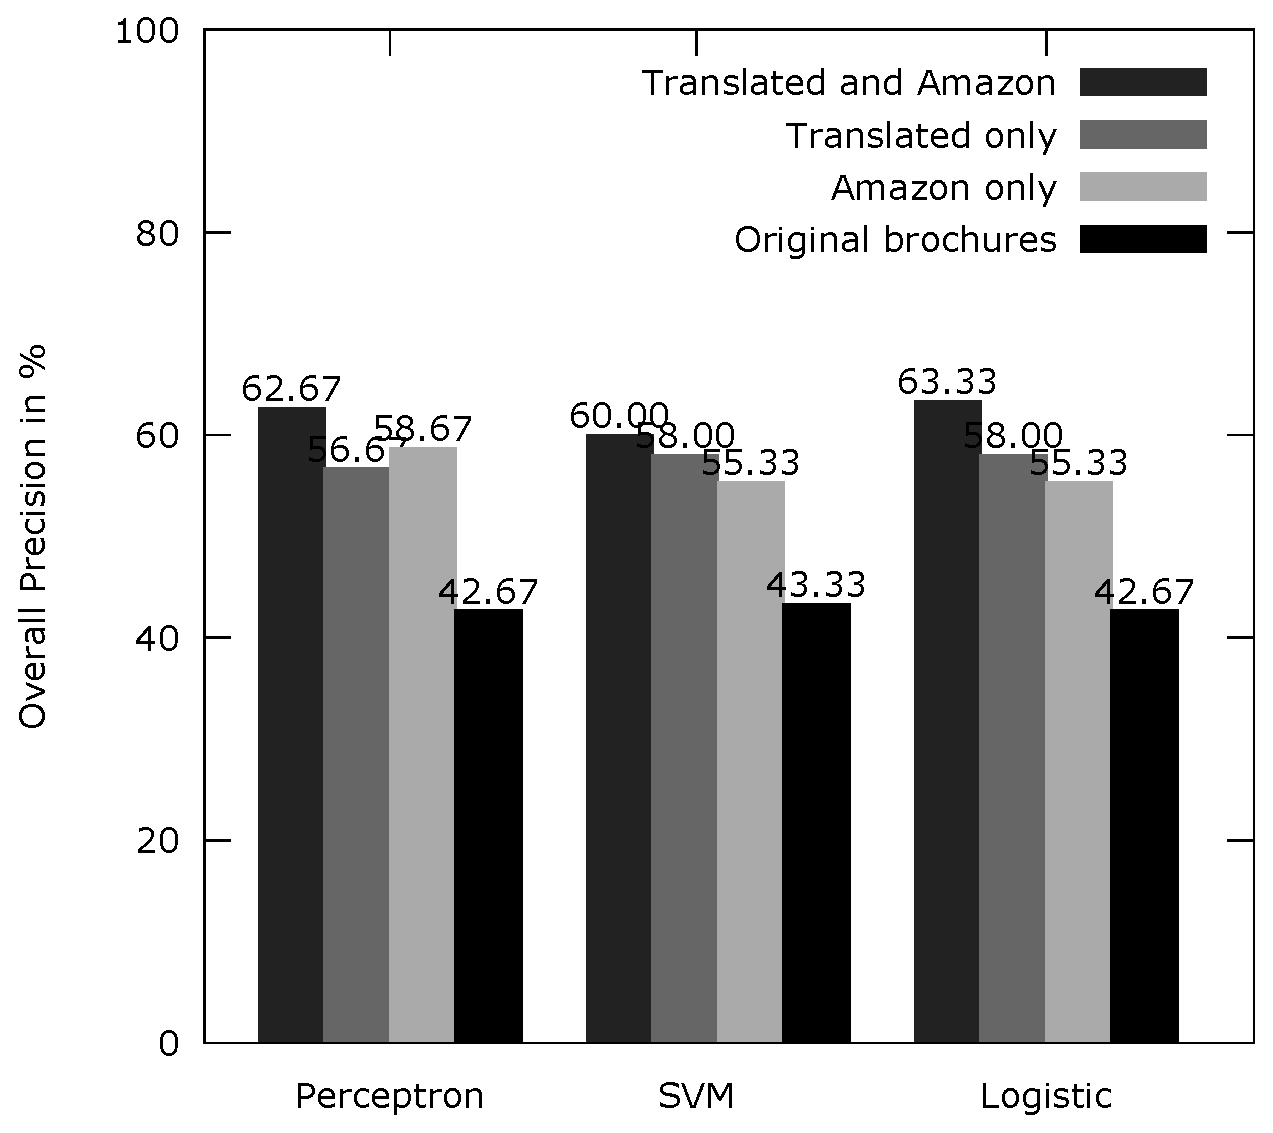
\includegraphics[width=\textwidth]{figures/product_translate_amazon_with_none.eps}
		\caption{with ``no-product'' prediction}
	\end{subfigure}~
	\begin{subfigure}[t]{0.5\textwidth}
		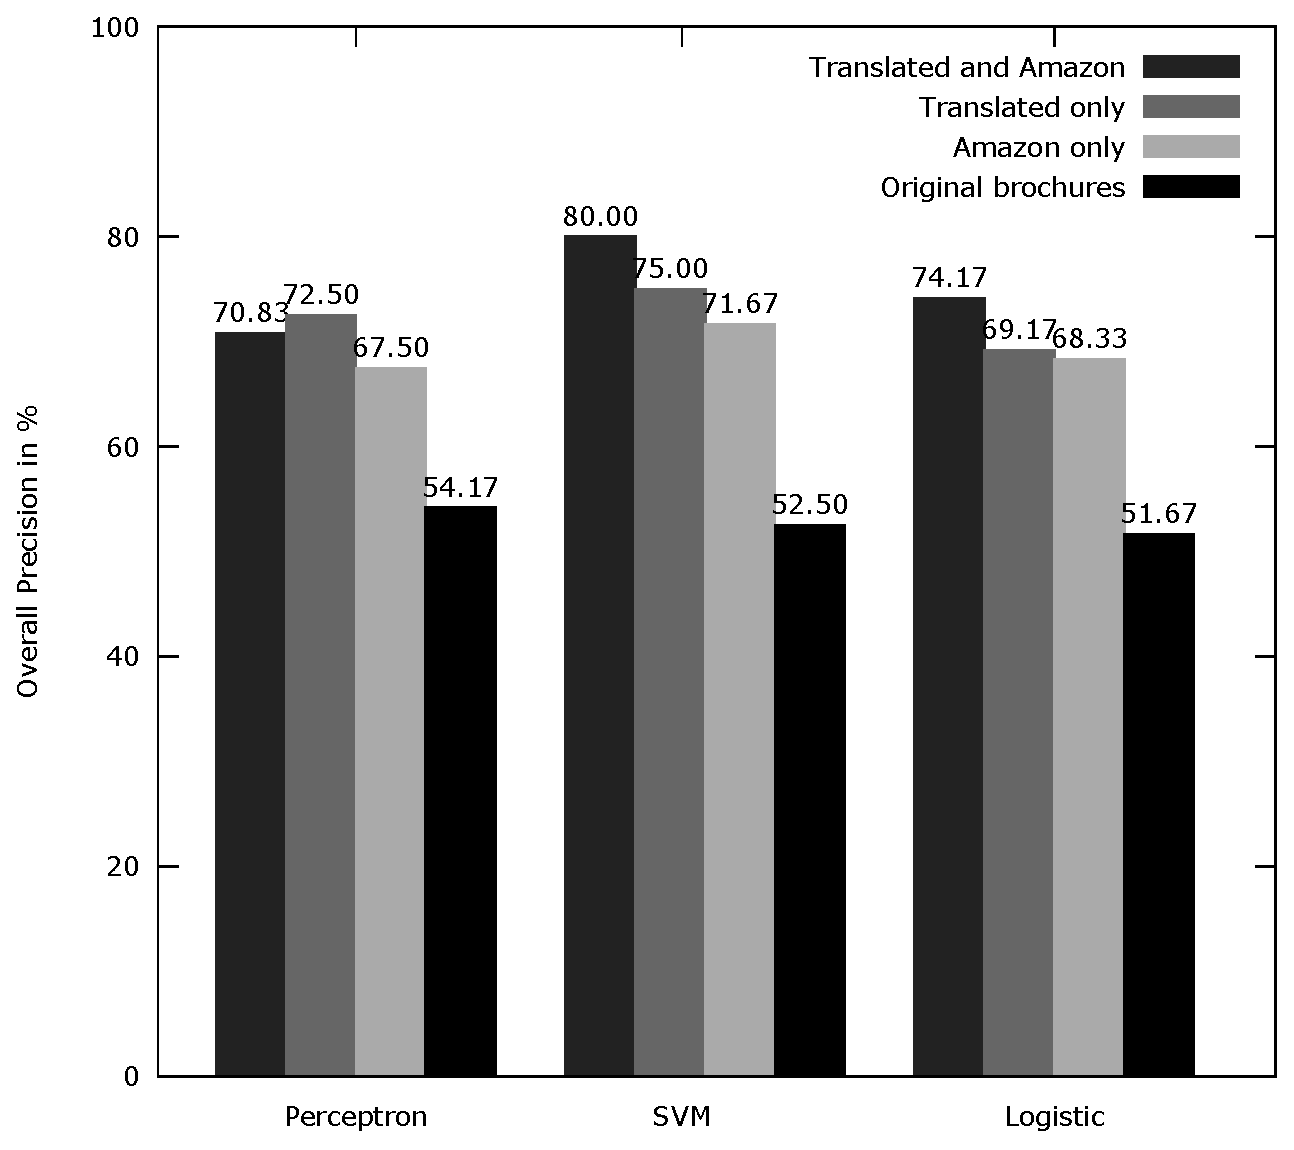
\includegraphics[width=\textwidth]{figures/product_translate_amazon_without_none.eps}
		\caption{without ``no-product'' prediction}
	\end{subfigure}
	\caption{Feature Selection: comparison of ten-, 100- and 1000-most occurred words selected as tf-idf features}
	\label{fig:product_translate_amazon}
\end{figure}

\subsection{Results}
\label{sub:results}

\subsubsection{Demand classifier}
\label{ssub:demand_classifier}

\begin{table}[h]
	\centering
	\begin{tabular}{lc}
		\hline
		\textbf{Metric} & \textbf{Result}  \\
		\hline
		\hline
		Precision of the demand classifier & 88~\% \\
		\hline
		Recall of the demand classifier & 51~\%  \\
		\hline
		Overall precision of the demand classifier & 93~\%  \\
		\hline
	\end{tabular}
	\caption{Cross validation results on demand classifier}
	\label{table:demand_evaluation}
\end{table}

\todo{WRITE HERE SOMETHING!}


\subsubsection{Product classifier}
\label{ssub:product_classifier}

As we said before, linear classifiers performed best for the product classification.
Because they only have a small difference, we will evaluate on three linear classifiers: logistic regression, perceptron, and support vector machines.
Comparing these classifiers with a naive \todo{naive approach? sounds like bashing them!} approach (K-Nearest-Neighbor classification) we can see a better performance as it is shown in figure \ref{fig:product_eval}.
In this figure you can see the four classifiers, which are predicting for each post exactly one of the four products.
Additionally to this ``forced'' prediction (the without ``no-product'' prediction) we have modified the linear classifiers in the way, that they predict for each post the four product if and only if one of the product predictions has a significantly greater probability.
In the other case, so if all products are predicted with quite equal probability, ``no-product'' is predicted as the product.
This classification mode is nearer to the real world scenario, since not every LinkedIn post we have crawled can be mapped to one of the product classes.
And as the figure \ref{fig:product_eval} shows, this approach increases the accuracy by about seven to ten percent.

For the final product classifier we have made some improvements, which are based on some design decisions.
We will introduce and evaluate two of these design decisions in the following subsections.

\subsubsection{Design decision 1: feature selection}
As already mentioned in the section \ref{sub:feature-selection}, we use for the product classifier the classical tf-idf feature selection.
Additionally we pick only the ten words with the highest tf-idf assuming, that these words describe the product best.
The comparison of the ten-best approach with the 100-best and 1000-best approaches you can see in the figure \ref{fig:product_feature_selection}
As you can see, both classification modes (with and without ``no-demand'' prediction), the ten-best feature selection performs best.

\subsubsection{Design decision 2: translation and book descriptions}
Section \ref{sub:initial_data_set} described our approach for enlargement and linguistic adaptation of the training set.
Compared with a naive approach, using the brochures as they are, the translation of the German brochures and the enlargement of the training brings an improvement of 17-20\% (for without-no-product mode) and 16-28\% (for the with-no-product mode) for the demand classifier as it is shown in the figure \ref{fig:product_translate_amazon}.
We can also see, that each of the steps, the translation and the enlargement, improves the performance.
So having same problems with other data sets, we assume that this design decision could improve any other classifier implementation in the same manner.

\subsection{Two stage classifier}
\label{sub:two_stage_classifier}

As we propose in our work to use a two stage classifier for the \nto problem.
To evaluate this approach we compare our two-stage classifier against just a one-stage classifier using the brochures as traning data.
This one-stage classifier is identical to our product classifier.

For that evaluation we have changed the test set annotations in the way, that if an annotated (our manual annotation) post was been classified as ``no-demand'', the product classification will be ignored, so it will be ``no-product''.
Thus we can compare the predictions of the product classifier (which are one of the products or ``no-product'') with the predictions of the two stage classifier (which are ``demand'' or ``no-demand'' and if ``demand'' then one of the products or ``no-product'').
Because the demand classifier is also trained on the LinkedIn posts, we have to do a cross validation on the LinkedIn posts, because otherwise, we would learn and train on the same data.
We have used a ten fold cross validation here.
The accuracy of the both classification you can see in Table \ref{table:two_stage_eval}.
As you can see, the two stage approach performs better than the single product classification.

\begin{table}
	\centering
	\begin{tabular}{c|c}
		\hline
		Product classification & Two stage classification \\ \hline \hline
		69.73\% & 81.35\% \\ \hline
	\end{tabular}
	\caption{Comparison of the standalone product classification with the two stage classification}
	\label{table:two_stage_eval}
\end{table}

\todo{To make it fair we better should evaluate our classifier against a one-stage classifier also using the demand post as training data.}
\todo{noch weiter ausführen, was das ergbniss nun heißt? und warum wir so gut sind? \\
--> Wir sind so gut, weil der product classifier alleine natürlich keine chance hat demand zu erkennen bzw zu lernen ...}

\todo{Fuer den einen Classifier geben wir alle rein, fuer den anderen splitten wir in Demand and Product.}


%!TEX root = ../paper.tex
\section{Conclusion and Future Work}

In this work we presented a new approach to online marketing.

Using a combination of supervised machine learning algorithms, we are able to find customers .

This work focused on business-oriented social networks, however the approach can also be adapted towards consumer-oriented networks like Facebook.
Users might ask for the best running shoes to buy, or where to buy the latest computer laptop.

\todo{What has to be done to enable active learning for the entire problem.}

\label{sec:conclusion}
\begin{itemize}
	\item Conclude your work by repeating the contributions
	\item Highlight the best evaluation results
	\item Identify future directions (what would be the next topic of the next paper?)
	\item Learning loop: iterative learning, use reuse salesmen tags
\end{itemize}


\newpage
\bibliographystyle{abbrv}
\bibliography{references}

\end{document}
